%-----------------------------------------------------------------------------------------------%
%
% % Oktober 2022
% Template Latex untuk Laporan Kerja Praktek Program Studi Sistem informasi ini
% Dikembangkan oleh Daffa Takratama Savra (daffatakratama13@gmail.com)

% Template ini dikembangkan dari template yang dibuat oleh Inggih Permana (inggihjava@gmail.com).

% Orang yang cerdas adalah orang yang paling banyak mengingat kematian.
%
%-----------------------------------------------------------------------------------------------%


%-----------------------------------------------------------------------------%
\chapter{\babTiga}
%-----------------------------------------------------------------------------%
\section{Waktu dan Tempat Pelaksaan Kerja Praktek}
Waktu	: Tanggal 03 Juli sampai dengan tanggal 01 September 2023

Tempat: Laboratorium Prodi Sistem Informasi

Alamat	: Jl. Soebrantas No. 155 KM 15, Pekanbaru 28293

%-----------------------------------------------------------------------------%
\subsection{Jadwal Kerja Praktek}
Pelaksanaan kegiatan dilakukan dalam kurun waktu 2 (dua) bulan terhitung sejak tanggal 03 Juli – 01 September tahun 2023. Jadwal kerja praktek dapat dilihat pada Gambar 3.1 berikut:

\begin{figure}
  \centering
  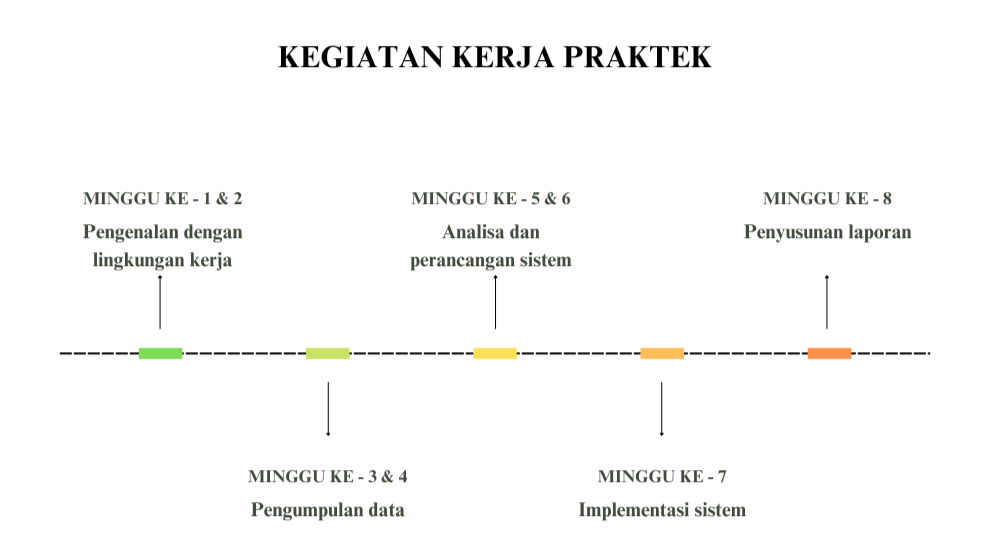
\includegraphics[width=0.82\linewidth]{konten//gambar/kegiatan kerja praktek.png}
  \caption{Kegiatan Kerja Praktek}
  \label{fig:enter-label}
\end{figure}
%-----------------------------------------------------------------------------%
\subsection{Uraian Kerja Praktek}
%-----------------------------------------------------------------------------%
Tugas kerja praktek ini dilaksanakan pada Laboratorium Sistem Informasi
UIN Suska Riau yang beralamatkan Jl. H.R. Soebrantas KM 15, Tuah Madani, Panam, Pekanbaru dalam kurun waktu 58 hari dihitung sejak 03 Juli 2023 sampai 01 September 2023. Kegiatan yang dilakukan disusun dalam proses perencanaan kerja, rencana tersebut adalah:
\begin{enumerate}
  \item Kegiatan pada minggu pertama dan kedua dilakukan agenda proses perkenalan dengan pegawai dan pembimbing kerja praktek di tempat kerja praktek. Perkenalan dilakukan pada tanggal 03 Juli 2023 mulai dari memperkenalkan diri kepada pegawai di tempat kerja praktek.
  \item Pada minggu ketiga dan keempat dilakukan proses pengamatan alur dan prosedur kerja, serta sudah mulai melakukan pengumpulan data dan pengolahan data dengan melakukan teknik pengumpulan seperti observasi dan wawancara yang di khususkan mengenai analisis dan perancangan sistem informasi.
  \item Pada minggu keempat dan kelima dilakukan proses analisa kebutuhan sistem yang diperlukan dari data yang diperoleh.
  \item Selanjutnya pada minggu keenam, ketujuh dan kedelapan yaitu melanjutkan perancangan dan sudah masuk ketahap pengkodingan dan implementasi sistem, sekaligus merupakan minggu perpisahan pada kerja praktek.
\end{enumerate}
%-----------------------------------------------------------------------------%
\section{Metodologi Kerja Praktek}
Metodologi berisi tahapan-tahapan yang dilakukan dalam penyusunan lapo-
ran kerja praktek. langkah – langkah yang ditempuh dalam melakukan penelitian ini
dapat dilihat pada Gambar 3.2 berikut.
\begin{figure}
  \centering
  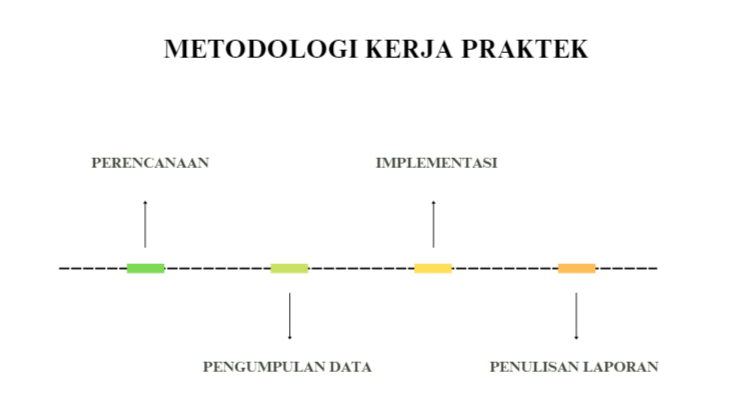
\includegraphics[width=0.82\linewidth]{konten//gambar/metodologi kerja praktek.png}
  \caption{Metodologi Kerja Praktek}
  \label{fig:enter-label}
\end{figure}
%-----------------------------------------------------------------------------%
% Isi sesuai keinginan
%-----------------------------------------------------------------------------%
\subsection{Tahap Perencanaan }
%-----------------------------------------------------------------------------%
Langkah pertama adalah menetapkan masalah yang akan dipecahkan, adapun langkah-langkah dalam perencanaan sebagai berikut:
\begin{enumerate}
  \item Mulai \\
        Merupakan tahapan awal dalam setiap kegiatan yang akan dilakukan.
  \item Menentukan Topik Penelitian \\
        Topik penelitian ditentukan dari uraian masalah dan kendala yang didapat dari observasi secara langsung di Laboratorium Sistem Informasi.
  \item Menentukan Masalah \\
        Setelah observasi dilakukan, untuk mendukung pencapaian kerja praktek ini maka selanjutnya dilakukan penentuan masalah agar bisa mendapat masalah untuk dipecahkan.
  \item Menentukan Tujuan Kerja Praktek \\
        Selanjutnya adalah penentuan tujuan dari Kerja Praktek ini, agar tujuan dalam penulisan Laporan Kerja Praktek lebih Jelas.
  \item Menentukan Metode Penelitian \\
        Agar hasil dari penelitian ini sesuai harapan maka dibutuhkan penentuan implementasi untuk mendukung penelitian ini yaitu menggunakan \textit{framework} CodeIgniter 4.
\end{enumerate}
%-----------------------------------------------------------------------------%
\subsection{Tahap Pengumpulan Data}
%-----------------------------------------------------------------------------%
Tahap ini adalah tahap penulis melaksanakan pengumpulan data Kerja Praktek, pada tahap ini yang dilakukan adalah:
\begin{enumerate}
  \item  Observasi \\
        Penulis melakukan pengamatan di Laboratorium Sistem Informasi secara langsung.
  \item  Wawancara \\
        Penulis melakukan wawancara langsung dengan Kepala Laboratorium Sistem Informasi UIN Suska Riau untuk mengajukan beberapa pertanyaan.
        % \item  Studi Pustaka \\
        % Studi pustaka dilakukan dengan cara mengambil literature yang berkaitan dengan materi. Pada tahapan pengumpulan data studi pustaka Penulis mengambil beberapa referensi dari buku, jurnal, ebook dan internet.
\end{enumerate}

% Data yang dikumpulkan adalah sebagai berikut:
% \begin{enumerate}
%     \item Data Primer \\
%     Data Primer adalah data yang diambil secara langsung dari sumber aslinya, melalui narasumber yang tepat dan dapat dijadikan data pembuatan laporan.
%     \item Sekunder
%     Data Sekunder adalah data yang diambil melalui jurnal, e-book dan juga buku-buku referensi dari berbagai penulis.
% \end{enumerate}
%-----------------------------------------------------------------------------%
% \subsection{Tahap Analisa dan Hasil}
% %-----------------------------------------------------------------------------%
% Tahap analisa dan perancangan dilakukan untuk membuat rancangan sistem yang baru dengan menganalisa data-data yang sudah didapatkan dari hasil pengumpulan data sebelumnya.
% \begin{enumerate}
%       \item Analisa sistem lama \\
%             Berdasarkan data-data yang telah didapatkan pada tahap pengumpulan data, maka dilakukan analisa sistem yang digunakan dalam proses pencatatan inventaris dimulai dari permasalahan yang terjadi saat proses pencatatan, peminjaman, dan cara mengatasi permasalahan yang terjadi.
%       \item Analisa sistem baru \\
%             Dari analisa sistem lama, maka dilakukan analisa dan rancangan sistem baru untuk mengatasi permasalahan dengan mengunakan metode yang dipilih pada tahapan perencanaan.
% \end{enumerate}
%-----------------------------------------------------------------------------%
\subsection{Tahap Implementasi}
%-----------------------------------------------------------------------------%
Pada tahap implementasi dilakukan pengkodingan untuk membangun sistem yang sudah dianalisa dan dirancang pada tahap sebelumnya.
\begin{enumerate}
  \item Mengimplementasikan sistem informasi inventaris laboratorium melanjutkan desain \textit{interface}, \textit{database}, dan UML yang sudah dilakukan pada tahap sebelumnya yang akan digunakan sebelum tahap pengkodingan.
  \item Melakukan kodingan sistem
        Melakukan pengkodingan sistem inventaris dengan rancangan yang telah dibuat dengan desain-desain yang telah dibuat sebelumnya.
\end{enumerate}
%-----------------------------------------------------------------------------%
\subsection{Tahap Penulisan Laporan}
%-----------------------------------------------------------------------------%
Tahap terakhir ini adalah melakukan penulisan laporan. Kegiatan yang dilakukan diantaranya melakukan konsultasi terhadap pembimbing, dokumentasi hasil kerja praktek hingga selesainya penulisan laporan.
%-----------------------------------------------------------------------------%